
\documentclass[preprint,12pt]{elsarticle}

\usepackage[spanish]{babel}
\usepackage{amssymb}
\usepackage{graphicx}
\usepackage{lineno}
\usepackage[utf8]{inputenc}
\usepackage{url}
\usepackage{natbib} 
\usepackage{amsmath} 
\usepackage{amssymb} 
\usepackage{graphicx}

\begin{document}
	
	\begin{frontmatter} 

		\title{\huge MAQUINAS VIRTUALES VS CONTENEDORES}
		
		\author{Huichi Contreras, Franklin Carlos            (2016056193)}
		\author{Huillca Umpiri, Willian              		  (2015053793)}
		\author{Robles Flores, Anthony Richard              (2016056192)} 
		\address{Escuela Profesional de Ingeniería de Sistemas}
		\address{Universidad Privada de Tacna}
		\address{Tacna, Perú}
		
%% ABSTRACT --------------------------------------------------------------------------------------------------------------------

		\begin{abstract}
In this article we will learn concepts, differences and uses of virtualization and containers, this will allow us to choose the most recommendable option for the performance of a system that is being developed or to make changes in it.\\
\textbf{Keywords:}  \\
 virtualization, containers, tools, processes, simulation, resources.\\

		\end{abstract}

%% ----------------------------------------------------------------------------------------------------------------------------------

	\end{frontmatter}

%% RESUMEN ---------------------------------------------------------------------------------------------------------------------

\section{Resumen}


En este artículo aprenderemos conceptos, diferencias y usos de la virtualizacion y contenedores, esto nos permitirá elegir la opción más recomendable para el desempeño de un sistema que se esté desarrollando o para realizar cambios en él.\\

\textbf{Palabras clave:}   \\
virtualizacion, contenedores, herramientas, simulacion, procesos, recursos.\\



%% ----------------------------------------------------------------------------------------------------------------------------------


%% INTRODUCION ----------------------------------------------------------------------------------------------------------------

\section{Introducción} 

Antes de ahondar en el concepto de contenedores, volvamos unos años atrás para recordar el nacimiento de la virtualización. A medida que el hardware se hacía más poderoso nos encontramos con que el software no ocupaba todas las capacidades de la maquina física donde se encontraba siendo ejecutada (en muchos casos ni siquiera una fracción de estos recursos). Dado lo anterior se crearon recursos “virtuales” para simular el hardware base sobre el cual se ejecuta el software, permitiendo que múltiples aplicaciones puedan ser ejecutadas al mismo tiempo, cada una usando una fracción de los recursos del hardware físico disponible. A a esta “simulación” que permite de compartir recursos la denominamos comúnmente “virtualización”.

La mayoría de nosotros cuando escuchamos el concepto de virtualización pensamos inmediatamente en máquinas virtuales, pero es importante entender que este es solo un tipo de virtualización en el cual se habilita un sistema operativo el cual tiene la ilusión de que posee recursos dedicados para operar. Entendiendo lo anterior podemos ahora definir a los Contenedores como creadores de la percepción de un ambiente aislado exclusivo para la aplicación mientras que en la virtualización “tradicional” de máquinas virtuales la aplicación se ejecuta en un sistema operativo virtualizado donde convive con otros aplicativos.


%% ----------------------------------------------------------------------------------------------------------------------------------


%% TITULO  ------------------------------------------------------------------------------------------------------------

\section{Marco teorico}

\subsection{¿Que es la virtualización?}
La virtualizacion es la creación de una versión virtual (no física) de algo. Esta basada en software, se puede aplicar a sistemas operativos, almacenamiento, servidores, aplicaciones, redes, etc. y es una manera de reducir gastos y aumentar eficiencia y agilidad en las empresas.

\subsubsection{Virtualizacion de servidores}
La virtualizacion de servidores ayuda a evitar ineficiencias ya que permite ejecutar varios  sistemas operativos en una maquina fısica con maquinas virtuales con acceso a los recursos de todos. Tambien permite generar un cl uster de servidores en un unico recurso para ası mejorar mucho mas la eficiencia y la reduccion de costes. Tambien permite el aumento de rendimiento de las aplicaciones y la disponibilidad al aumentar la velocidad en la carga de trabajo.

\subsubsection{Virtualizacion de escritorios}
La implementacion de escritorios virtualizados permite ofrecer a las sucursales o empleados externos de forma rapida y sencilla un entorno de trabajo y una reduccion de la inversion a la hora de gestionar cambios en estos.

\subsubsection{Virtualizacion de red}
Se trata de reproducir una red fısica completa mediante software para poder ejecutar los mismos servicios que una red convencional y sus dispositivos. Cuentan con las mismas caracterısticas y garantıas que las redes fısicas con las ventajas que nos ofrece la virtualizacion ademas de la liberacion del hardware.

\subsubsection{Almacenamiento definido por software}
La virtualizacion del almacenamiento permite prescindir de los discos de los servidores. Los combina en depositos de almacenamiento de alto rendimiento y los distribuye como software. Este nuevo modelo permite aumentar la eficiencia en el guardado de datos.

\subsection{Ventajas de la virtualizacion}
Como se ha podido apreciar en los tipos de virtualizacion presentados anteriormente, esta conlleva una mejora considerable tanto en el rendimiento, agilidad, flexibilidad, escalabilidad, etc. como en una reduccion considerable de los costes economicos y de tiempo y una simplificacion en la gestion de la infraestructura.
\begin{itemize}
\item Reduce los costes de capital y los gastos operativos.
\item Minimiza o elimina los tiempos de inactividad
\item Aumenta la productividad, la eficiencia, la agilidad y la capacidad de respuesta
\item Implementa aplicaciones y recursos con mas rapidez. 
\item Garantiza la continuidad del negocio y la recuperacion ante desastres.
\item Simplifica la gestion del centro de datos.
\end{itemize}

\subsection{Contenedores}
\par Un contenedor de software se puede considerar como una aplicación para el servidor. Estos se encargan de proporcionar a las aplicaciones archivos, variables y biblotecas que sean necesarios para ejecutarse y maximiza su portabilidad.
Para poder instalar una aplicación, el contenedor se carga en el ordenador en un formato portable o imagen (Image) que incluye todos los datos necesarios para su funcionamiento y, en el ordenador, se inicia en un entorno virtual. {know}
Los contenedores permiten que estos equipos de desarrollo alcancen una eficiencia muy alta en la entrega y el despliegue de software, al solucionar muchos de los retos que presenta la virtualización tradicional.
\par Beneficios:
	\begin{itemize}
		\item Ahorro de espacio y consumo. No se tendrá la necesidad de crear maquinas virtuales en las que instalarlas.
		\item Reutilización. Se puede crear tantas instancias como necesitemos, destruirlas y reproducir el entorno inicial.
		\item No "ensucia". No se tendrá que instalar dentro de nuestro equipo con la problemática que ello conlleva en algunos casos.
		\item Compartir. Estas imágenes las podremos distribuir comodamente entre los componentes de nuestro equipo.
		\item Se obtiene mayor modularidad. El desarrollo con contenedores es ideal para un enfoque basado en microservicios para el diseño de aplicaciones.{campus}
	\end{itemize}
\par Ventajas de los contenedores: \\
Los contenedores de aplicaciones “empaquetan” los recursos necesarios para el funcionamiento de una aplicación sin embargo, las mayores ventajas de tales contenedores radican, sobre todo, en la gestión y en la automatización de software basado en contenedores.{know}
\begin{itemize}
		\item Instalación más sencilla: los contenedores de software se inician a partir de imágenes o representaciones portables de un contenedor, incluyendo un programa y todos los componentes requeridos. De esta manera se compensan las diferencias entre sistemas operativos. Su instalación se reduce a la introducción de una línea de comando.
		\item Independiente de la plataforma: las imágenes se pueden transportar cómodamente de un sistema a otro y se caracterizan por una considerable independencia de la plataforma. Lo único que se necesita para iniciar un contenedor desde una imagen es un sistema operativo que soporte contenedores.
		\item Pérdidas por virtualización mínimas: con un Linux y Docker container, la instalación de contenedores requiere alrededor de 100 MB y unos pocos minutos, aunque no es solo esto a lo que se oponen los administradores de sistemas. Mientras que la virtualización de hardware trae consigo una pérdida de rendimiento para el hipervisor y otros sistemas operativos, los contenedores, al prescindir de todo esto, reducen esta pérdida al mínimo.
		\item Aplicaciones aisladas: cada programa funciona independientemente de otros contenedores, de forma que aplicaciones con requerimientos opuestos pueden funcionar en paralelo en el mismo sistema.
		\item Administración y automatización unitarias: debido a que en una plataforma como Docker todos los contenedores son gestionados con las mismas herramientas, es posible automatizar todas las aplicaciones de manera centralizada. Por esto, estas soluciones están indicadas sobre todo para arquitecturas de servidor en las cuales los componentes están distribuidos en varios servidores, de forma que se carga con los pesos de instancias diferentes. En estos ámbitos de aplicación, el Docker container dispone de herramientas con las cuales configurar automatismos. Esto posibilita, por ejemplo, iniciar instancias nuevas de forma automática en momentos puntuales de sobrecarga. \\
\end{itemize}
\par Al final, el uso de los contenedores es muy conveniente, tambien puede traer un nivel bajo de seguridad estariamos dejando de usar sistemas operativos separados. Pues, los contenedores no son tan herméticos como las máquinas virtuales con sistema operativo propio. En consecuencia, aunque los contenedores constituyen una alternativa para la virtualización de hardware, de momento no la pueden sustituir por completo.\\

%% ----------------------------------------------------------------------------------------------------------------------------------

\section{Funcionamiento de Docker}

\subsection{Arquitectura}
Docker usa una arquitectura cliente servidor. El cliente de Docker se comunica con el Daemon de Docker para crear, ejecutar y distribuir los contenedores. 
Tanto el cliente como el Daemon pueden estar en el mismo sistema o pueden conectarse remotamente. 
Como Docker usa el kernel de Linux para su ejecucion, si el sistema operativo del sistema no es
este, se deber a usar una pequeña capa extra en la arquitectura de tipo VM (boot Docker) 
para poder correr Docker en la maquina.

\subsection{ Cliente de Docker}
Es la principal interfaz de usuario para Docker. Acepta los comandos del usuario y se comunica con el Daemon de Docker.

\subsection{ Imagenes de Docker (Docker Images)}
Las imagenes de Docker son plantillas de solo lectura, que nos permitiran crear contenedores basados en su configuracion.

\subsection{ Registros de Docker (Docker Registries))}
Los registros de Docker guardan las imagenes.  Estos son repositorios publicos o privados donde se pueden subir o descargar imagenes. Seríıa similar a GitHub para imagenes de Docker (Docker Hub).



\section{Creacion de Imagenes}
Como se comenta en el punto anterior, las imagenes de Docker son las plantillas para poder levantar los contenedores. Por eso la importancia de saber crear imagenes y personalizarlas ya que solo permiten lectura y los cambios que hagamos en los contenedores no se veran reflejados en  estas.
\\
La manera mas sencilla de crear una imagen es descargarla del Docker Hub con el comando explicado anteriormente:
\\

\begin{figure}[htb]
	\begin{center}
		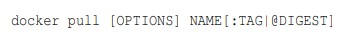
\includegraphics[width=14cm]{./IMAGENES/foto3} 
		
	\end{center}
\end{figure}

Este comando nos permite descargar una imagen en una version concreta o tag dependiendo de nuestras necesidades. Por defecto, si no se pone nada, descargara la ultima.

\begin{figure}[htb]
	\begin{center}
		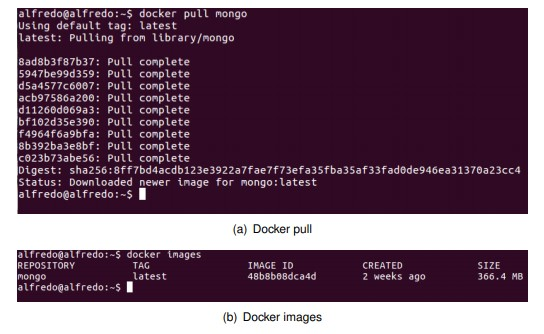
\includegraphics[width=14cm]{./IMAGENES/foto4}
		
	\end{center}
\end{figure}

En la figuras podemos apreciar como se descarga la ultima version de la imagen de MongoDB y nos genera la imagen.
Una vez obtenida la imagen se pasara a levantar el contenedor para poder ejecutar el servicio con otro de los comandos explicados.


\begin{figure}[htb]
	\begin{center}
		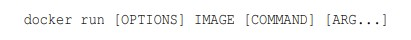
\includegraphics[width=14cm]{./IMAGENES/foto5}
		
	\end{center}
\end{figure}

\begin{figure}[htb]
	\begin{center}
		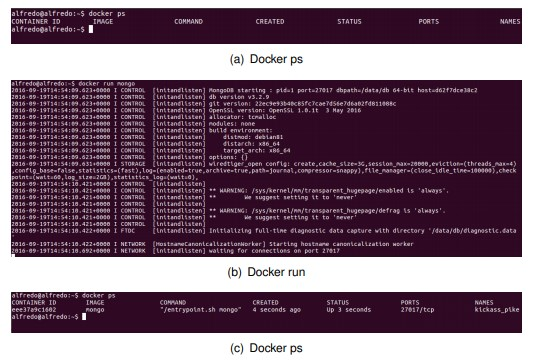
\includegraphics[width=14cm]{./IMAGENES/foto6}
		
	\end{center}
\end{figure}

En la figuras 2.4 se puede apreciar como utilizando el comando docker ps que permite ver que contenedores estan levantados, no hay ninguno (a) y como al inicializar con el comando docker run mongo levanta el servicio (b) y esta vez sí aparece el contenedor
(c).


La segunda manera de crear y personalizar imagenes es mediante un  DockerFile, que es un documento de texto donde se encuentran los comandos que se deben ejecutar para generar nuestra imagen.

El comando docker build comunica al Daemon de Docker que debe de leer el DockerFile del directorio actual y seguir las instrucciones linea por linea para la creacion de nuestra imagen. Este proceso va pintando los resultados por pantalla y generando imagenes intermedias para obtener asi  una cache que nos permitira en caso de errores, una vez corregido el DockerFile, continuar desde el punto conflictivo.

\begin{figure}[htb]
	\begin{center}
		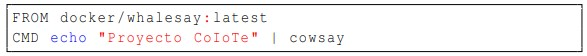
\includegraphics[width=14cm]{./IMAGENES/foto7}
		
	\end{center}
\end{figure}

Aqui tenemos un ejemplo sencillo de DockerFile que nos servira para explicar de una manera rapida como crearlos.

FROM indica la imagen base que va a utilizar para seguir futuras instrucciones. Buscara si la imagen se encuentra localmente, en caso de que no, la descargara. En nuestro ejemplo utiliza la ultima version de la imagen docker/whalesay. 

\section{Docker Compose}
Docker Compose es un orquestador que nos permite ejecutar aplicaciones que utilicen varios contenedores a la vez. Se creara un archivo docker-compose.yml donde se configuraran todos los servicios necesarios para nuestra aplicacion. Una vez ejecutado este archivo nos generara todas las imagenes y con estas los contenedores especificados a la 
vez que arrancara la aplicacion.
\\
Los comandos que se utilizaran seran similares a los utilizados en la creaci on de imagenes.
\\
Para ejecutar el servicio y levantar todos los contenedores.

\begin{figure}[htb]
	\begin{center}
		
\includegraphics[width=14cm]{./IMAGENES/foto8}
		
	\end{center}
\end{figure}

Para detener el servicio y detener los contenedores.

\begin{figure}[htb]
	\begin{center}
		
\includegraphics[width=14cm]{./IMAGENES/foto9}
		
	\end{center}
\end{figure}



%% CONCLUSIONES------------------------------------------------------------------------------------------------------------
\section{Conclusiones}\label{sec:6}


\begin{itemize}
	\item Los Contenedores son un método de virtualización de un sistema operativo que permite ejecutar una aplicación junto con sus elementos dependientes, en un ambiente aislado e independiente.
	\item La virtualizacion lo que hace es crear a traves del software una version virtual de un recurso, como virtualiza de manera completa un software, consume los recursos del hardware tal como lo hicieramos en una maquina física reduciendo el rendimiento y el performance de la maquina que aloja a la virtual
\end{itemize}


%% ----------------------------------------------------------------------------------------------------------------------------------






%%  REFERENCIAS BIBLIOGRÁFICAS  (OJO NO TOCAR CON CITEP SOLO SE PONEN)------------------------------------------------------------------------------------------
	
	\newpage
	
	\bibliographystyle{apalike} 	%ESTILO
	%%\bibliography{BIBLIOGRAFIA}	 
	
	
\end{document}
